\documentclass[border=10pt]{standalone}
\usepackage{tikz}
\usetikzlibrary{automata, positioning, arrows.meta}

\begin{document}
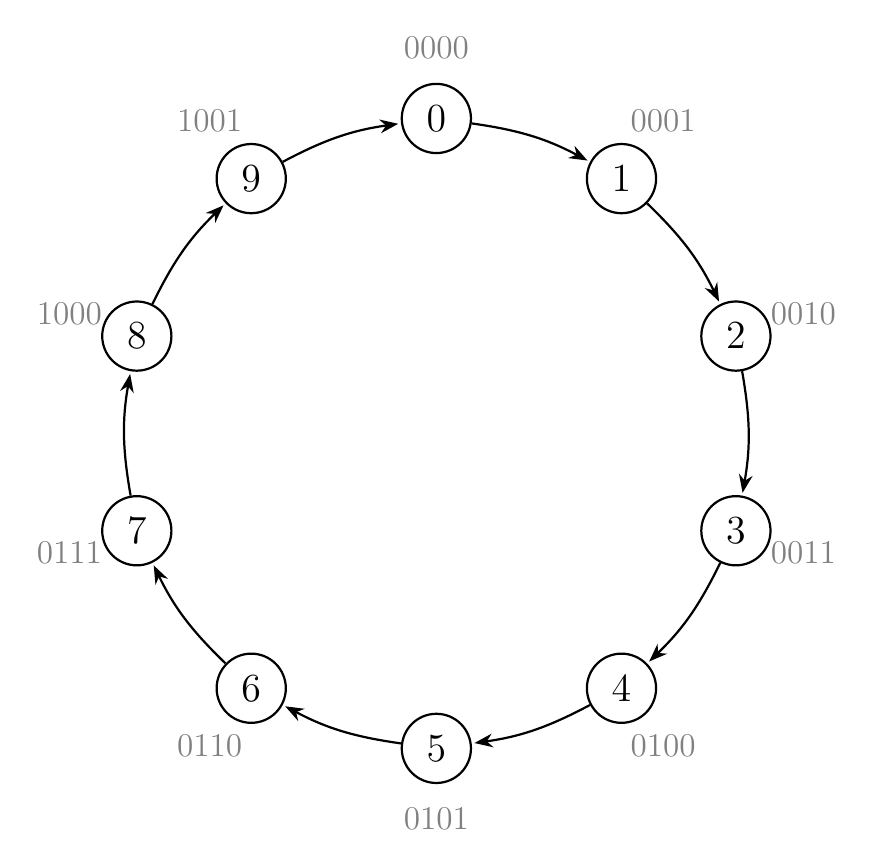
\begin{tikzpicture}[
    ->, >=Stealth, 
    shorten >=1pt, 
    auto, 
    node distance=2.5cm, 
    thick
]

    % Circular layout for states 0-9
    \def\radius{4.0cm}
    \def\n{10} % Number of states
    
    \foreach \i in {0,...,9} {
        % Angle: 90 degrees is top (0), clockwise is negative angle
        % 360/10 = 36 degrees per step
        % Start at 90 (Top) -> 0
        \pgfmathsetmacro{\angle}{90 - \i * 36}
        \node[state,font=\Large] (s\i) at (\angle:\radius) {\i};
    }
    
    % Transitions
    \path (s0) edge [bend left=10](s1)
          (s1) edge [bend left=10](s2)
          (s2) edge [bend left=10](s3)
          (s3) edge [bend left=10](s4)
          (s4) edge [bend left=10](s5)
          (s5) edge [bend left=10](s6)
          (s6) edge [bend left=10](s7)
          (s7) edge [bend left=10](s8)
          (s8) edge [bend left=10](s9)
          (s9) edge [bend left=10](s0);

    % Optional: Add binary values near nodes?
    % Let's stick to decimal for clarity as primary, maybe small binary label outside?
    % BCD 0-9: 0000 to 1001. A label is nice.
    
    \foreach \i/\bin in {0/0000, 1/0001, 2/0010, 3/0011, 4/0100, 5/0101, 6/0110, 7/0111, 8/1000, 9/1001} {
        \pgfmathsetmacro{\angle}{90 - \i * 36}
        % Position label radially outside
        \node[font=\large, color=gray] at (\angle:\radius+0.9cm) {\bin};
    }

\end{tikzpicture}
\end{document}
